\documentclass[aspectratio=169]{beamer}
%\usetheme{Warsaw}
%AnnArbor, CambridgeUS, 
%\usecolortheme{beaver}
%\usetheme{seahorse}
\usetheme{Madrid}
%t\definecolor{pistachio}{rgb}{0.55, 0.77, 0.65}
%\definecolor{palecopper}{rgb}{0.85, 0.54, 0.4}
\definecolor{airforceblue}{rgb}{0.36, 0.54, 0.66}
%\definecolor{ashgrey}{rgb}{0.7, 0.75, 0.71}
%\definecolor{cadetgrey}{rgb}{0.57, 0.64, 0.69}
\usecolortheme[named=airforceblue]{structure} % Sample dvipsnames color

\setbeamercolor{block title alerted}{bg=white, fg=white} % 1- Block title (background and text)
\setbeamercolor{block body alerted}{bg=cadetgrey, fg=white} % 2- Block body (background)
\setbeamercolor{block title example}{bg=cadetgrey, fg=white} % 1- Block title (background and text)
\setbeamercolor{block body example}{bg=cadetgrey!25} % 2- Block body (background)
\setbeamercolor{block title}{bg=black!60,fg=white}

\setbeamersize{text margin left=20pt, ,text margin right=20pt} 

\usepackage[utf8]{inputenc}
\usepackage[portuguese]{babel}
\usepackage{graphicx}
%\usepackage{newtxtext,newtxmath}
\graphicspath{{imagens/}}
\usepackage{threeparttable}
\usepackage{tikz}
\geometry{}
\usepackage{multirow}
\usepackage{ragged2e}
\usepackage{subfig}
\usepackage{multicol}
\usepackage{booktabs}
\usepackage{tabularx}
\setbeamertemplate{itemize item}[square]
\setbeamertemplate{itemize subitem}[circle]
\setbeamertemplate{itemize subsubitem}[circle]
\setbeamercolor{itemize item}{fg=gray}
\setbeamercolor{itemize subitem}{fg=gray}
\setbeamercolor{itemize subsubitem}{fg=gray}
\setbeamertemplate{enumerate items}[square]
\setbeamercolor{item projected}{bg=gray!70!black,fg=white}
\usepackage[font=footnotesize,labelfont=bf]{caption}

\begin{document}
\title[Defesa TCC]{Concentrações regionais do seguro rural no Brasil em 2019}

\author[Walef Machado de Mendonça]{Walef Machado de Mendonça\\[3mm] Profª. Drª. Patrícia de Siqueira Ramos}
%\institute{}
\date{6 de Abril de 2022}

\begin{frame}{}
	\titlepage
	\begin{center}
	\footnotesize
	    Universidade Federal de Alfenas -- UNIFAL-MG
	\end{center}
\end{frame}


\section{Organização}


\section{Introdução}

\begin{frame}{Introdução}
\vspace{0.5cm}
		\begin{itemize}
		    \item A parcela da participação do agronegócio no PIB brasileiro foi de $20,5\%$ em $2019$ e em $2020$ este percentual chegou à $26,6\%$  (CEPEA, 2021).
		    \vspace{0.5cm}
		    \item  Em $2021$ a participação do agronegócio nacional deve ficar em torno de $30\%$ do PIB (CEPEA, 2021).
		    \vspace{0.5cm}
		    \item Entre $2006$ e $2017$, houve um acréscimo de cerca de $5,8\%$ na área total dos estabelecimentos agropecuários (IBGE, 2019).
		\end{itemize}
\end{frame}
\begin{frame}{Introdução -- Seguro rural}
	%\vspace{0.3cm}
	\begin{enumerate}
		\item Ambiente de elevado risco e grande incerteza.
		\begin{itemize}
		    \item Riscos de produção: instabilidades climáticas e ameaças sanitárias
		    \item Riscos de mercado: variações das taxas de câmbio e juros
		\end{itemize}
		\vspace{0.25cm}
		\item Oscilações na renda do setor.
		\vspace{0.25cm}
		\item Gerenciamento de risco -- contratação de Seguro Rural
		\begin{itemize}
		    \item  Amenizar as perdas e possibilita a recuperação da capacidade financeira do produtor
		    \item Ambiente mais favorável ao desenvolvimento das atividades agropecuárias 
		    \item Garantia do fluxo de renda aos produtores
		    \item Favorece um aumento da área plantada e facilita a obtenção de financiamento.
		\end{itemize}
	\end{enumerate}
\end{frame}

\begin{frame}{Introdução -- Programa de Subvenção ao Prêmio do Seguro Rural}
    \begin{enumerate}
        \item Problemas à consolidação do Seguro Rural:
            \begin{itemize}
                \item Elevados investimentos
                \item Custos administrativos
                \item Dependência espacial dos riscos
                \item Risco Moral
                \item Seleção adversa na formação das carteiras
            \end{itemize}
        \vspace{0.25cm}
        \item Programa de Subvenção ao Prêmio do Seguro Rural (PSR), instituído pela Lei 10.823/2003 e decreto no 5.121/2004
		(BRASIL, 2018)
            \begin{itemize}
                \item Mecanismo de estímulo para o desenvolvimento do seguro rural.
                \item Busca tornar o seguro rural mais acessível aos produtores.
                \item Divide os custos de aquisição da apólice entre o governo e os produtores. 
            \end{itemize}
    \end{enumerate}
\end{frame}


\subsection{Objetivos}

\begin{frame}{Objetivos} 
	\begin{block}{}
	    Identificar grupos de municípios com características semelhantes em relação à adesão ao seguro rural através do agrupamento de dados multivariados com base em medidas locais de autocorrelação espacial.
	\end{block}
\end{frame}

\subsection{Análise espacial}

\begin{frame}{Matriz de ponderação espacial}
	\begin{itemize}
	    \item É uma medida de proximidade entre as regiões.
	    \item Para um conjunto de $n$ áreas é definida como: 
	    \begin{align*}
        	\boldsymbol{W} =
	        \left[
	        \begin{array}{cccc}
		        w_{11} & w_{12} & \dots & w_{1n} \\
		        w_{21} & w_{22} & \dots &w_{2n} \\
		        \vdots & \vdots & \ddots & \vdots \\
		        w_{n1} & w_{n2} & \dots & w_{nn}\\
	        \end{array}
	        \right],
        \end{align*}
        \noindent Cada elemento $w_{ij}$ representa uma medida de proximidade entre as áreas $i$ e $j$. 
        \[
            w_{ij} = 
            \begin{cases}
                \text{1,} & \quad\text{se $i$ e $j$ são contíguos} \\
                \text{0,} & \quad\text{se $i$ e $j$ não são contíguos.}\\
            \end{cases}
        \]
        \noindent Por convenção, $w_{ij}=0,\quad \forall i=j$
	\end{itemize}
\end{frame}

\begin{frame}{\textit{I} de Moran}
	O \textit{I} de Moran mede a relação do desvio padronizado de uma variável $z$ numa área $i$ com o desvio padronizado das 	áreas vizinhas $j$ para a mesma variável $z$ (ALMEIDA, 2012).
	
	\begin{block}{}
		\small
		\begin{align}
		\label{IMoran}
		I = \dfrac{n}{S_0} \dfrac{\displaystyle\sum_{i} \sum_{j} w_{ij} z_i z_j}{\displaystyle\sum_{i=1}^{n} z_i^2}.
		\end{align}
		\noindent \small em que $z_i = (x_i - \bar{x})$, $w_{ij}$ é uma medida de contiguidade entre $i$ e $j$,  $n$ é o número de regiões e $S_0$ é a soma dos pesos espaciais ($w_{ij}$)
	\end{block}	
\end{frame}

\begin{frame}{Autocorrelação espacial local}
	\begin{itemize}
		\item Estatísticas globais fornecem padrões de associação espacial em todo o conjunto de dados
		\item Medidas de autocorrelação local buscam identificar padrões no interior de uma região de estudo  
		\item Podem informar a existência de um \textit{cluster} de valores autocorrelacionados em nível local
		\item Podem informar sobre existência de \textit{outliers} locais
		\item Para Anselin (1995), um indicador local de associação espacial (\textit{LISA}) deve satisfazer a dois critérios:
		\vspace{0.25cm}
		\begin{enumerate}
			\item Deve indicar clusters espaciais estatisticamente significativos;
			\item A soma dos indicadores locais deve ser levar ao indicador global.
		\end{enumerate}
	\end{itemize}
\end{frame}

\begin{frame}{\textit{I} de Moran local}
	Um indicador local de associação espacial do tipo \textit{LISA} é o \textit{I} de Moran local que é expresso por: 
	\begin{block}{}
		\small
		\vspace{0.25cm}
		\begin{align*}
		I_i = z_i \sum_{j}^{} w_{ij} z_j,
		\end{align*}
		\noindent \small em que $z_i$ e $z_j$ são os valores da variável padronizada nas regiões $i$ e $j$, $w_{ij}$ é uma matriz de pesos espaciais.
	\end{block}	
\end{frame}

\begin{frame}{G de Getis \& Ord}
    De acordo com Getis e Ord (1992), essa estatística indica a presença de agrupamentos localizados de concentração espacial, chamados de \textit{hot spots} e \textit{cool spots}. Para uma determinada variável $y$, a estatística é calculada da seguinte forma:
    
    \begin{block}{}
    \begin{align*}  
    G_i(d) = \dfrac{\sum_{j} w_{ij}(d) y_j}{\sum_{j}  y_j},\quad \text{para  $j \neq i$}.    
    \end{align*}
    O somatório em $j$ faz com que apenas os valores dos vizinhos próximos da região $i$ sejam utilizados no cálculo da estatística. 
    \end{block}
    
    A inferência a respeito da significância da estatística $G_i$ é baseada na normal padrão, ou seja, $Z(G_i)$. 
\end{frame}

\subsection{Análise multivariada}

\begin{frame}{Técnicas hierárquicas aglomerativas - método de \textit{Ward}}
     Este método se fundamenta na mudança de variação entre os grupos e também dentro dos grupos que são formados em cada passo do algoritmo. 
     
     A cada passo de agrupamento é calculada a soma de quadrados dentro dos grupos. A soma de quadrados dentro do $i$-ésimo grupo é definida como:  
    \begin{block}{}
    \begin{align*}
    SQDG_i = \sum_{j=1}^{n_i}(X_{ij} - \bar{X}_{i})^2,
    \end{align*}
    sendo $n_i$ o número de elementos no grupo $i$, $X_{ij}$ o vetor de observações do $j$-ésimo elemento amostral pertencente ao $i$-ésimo agrupamento e $\bar{X}_{i}$ o centróide do $i$-ésimo agrupamento, representando a soma de quadrados correspondente a tal grupo.
    \end{block}

\end{frame}

\begin{frame}{Técnicas hierárquicas aglomerativas - método de \textit{Ward}}
    A distância entre dois grupos quaisquer, $G_i$ e $G_l$, é definida como:
    
    \begin{block}{}
    \begin{align}\label{dist_g}
    d_{ G_i,G_l} = \left(\dfrac{n_l n_i}{n_l + n_i}\right)(X_{ij} - \bar{X}_{i})^2.		
    \end{align}
    \end{block}
    
    Em cada iteração do algoritmo, os dois grupos que minimizam a distância em (\ref{dist_g}) são combinados (MINGOTI, 2010).
    % Este método geralmente produz agrupamentos com aproximadamente o mesmo número de elementos em cada grupo e é adequado apenas para variáveis quantitativas por se baseado na comparação do vetor de médias amostral
\end{frame}

\begin{frame}{Técnica não hierárquica -- método das \textit{k}-médias}
    Este método busca por uma partição das $n$ observações em $k$ agrupamentos em que $k$ é dado por algum critério numérico de minimização. 
    
    A implementação mais utilizada do método das $k$-médias tenta encontrar a partição dos $n$ elementos em $k$ grupos que minimize a soma de quadrados dentro dos grupos ($SQDG$) em relação a todas as variáveis. Esse critério pode ser escrito como 
    
    \begin{block}{}
    \begin{align*}
    SQDG = \sum_{j=1}^{p}\sum_{l=1}^{k}\sum_{i \in G_l}(X_{ij} - \bar{X}_{j}^{(l)})^2,
    \end{align*}
    em que $\bar{X}_{j}^{(l)} = \displaystyle\frac{1}{n_i}\sum_{i \in G_l}X_{ij}$ é a média dos indivíduos no grupo $G_l$ em relação à variável $j$ (EVERITT; HOTHORN, 2011).
    \end{block}
\end{frame}

\subsection{Material e Métodos}

\begin{frame}{Material e métodos -- Dados}
	Dados de apólices de seguro rural dos municípios brasileiros em 2019. 
	\vspace{0.5cm}
    \begin{itemize}
        \item $5570$ Municípios
        \item $7$ variáveis
        \item \textit{Shapefile} dos municípios brasileiros. (IBGE, 2020).
        \item $373$ divergências relacionadas à distritos e outras localidades.
        \begin{itemize}
            \item Dados divergentes foram atribuídos aos municípios geograficamente mais próximos. 
        \end{itemize}
        \item Plataforma Atlas do Seguro Rural e Ministério da Agricultura, Pecuária e Abastecimento.
    \end{itemize}
\end{frame}

\begin{frame}{Material e métodos -- Variáveis}
    \begin{center}
    \small
        \begin{tabular}{ll}
            \hline 
            Sigla & Variável  \tabularnewline
            \hline 
            Total de apólices contratadas                  & TAC       \\ % ap\_contrat   
            Soma da importância segurada (R\$ milhão)      & SIS       \\ % t\_segurado   
            Soma dos prêmios (R\$ milhão)                  & SPR       \\ % soma\_premio  
            Total de subvenção (R\$ milhão)                & TSB       \\ % t\_subvencao  
            Soma das indenizações pagas (R\$ milhão)       & SIP       \\ % inde\_pagas   
            Taxa média aplicada às apólices                & TMA       \\ % tx\_media     
            Número de apólices indenizadas                 & NAI       \\ % ap\_indeniz 
            %\tabularnewline
            \hline 
            \vspace{0.1cm}
            \footnotesize{Fonte: Elaboração própria}
            \end{tabular}
    \end{center}    
\end{frame}

\begin{frame}{Material e métodos -- Procedimento de análise}
    \begin{enumerate}
        \begin{enumerate}
            \item Dada uma matriz de pesos espaciais $W$, calcule para cada variável a estatística \textit{G} de Getis-Ord local. Seja $z(G_j(x_i))$ a estatística resultante de para a $j-$ésima variável no $i-$ésimo município; 
            \vspace{0.5cm}
            \item Reúna os valores do passo anterior em uma matriz $Z$ de dimensão $(n \times p)$. Cada coluna de $Z$ expressa o padrão de autocorrelação local para uma variável, enquanto cada linha de $Z$ fornece o perfil de agrupamento em torno de cada unidade local; 
            \vspace{0.5cm}
            \item Aplique o método de \textit{Ward} no conjunto $Z$ de novas variáveis para especificar o número de grupos a ser utilizado no método das $k$-médias;
	        \vspace{0.5cm}
	        \item Aplique o algoritmo $k$-médias no conjunto $Z$. Esta etapa permite agrupar observações com base em seus perfis espaciais multivariados que contêm informações de localização e das variáveis.
\end{enumerate}
    \end{enumerate}
\end{frame}

\subsection{Resultados}

\begin{frame}{Resultados -- Distribuição espacial}
    \begin{figure}[h]
    	\centering
    	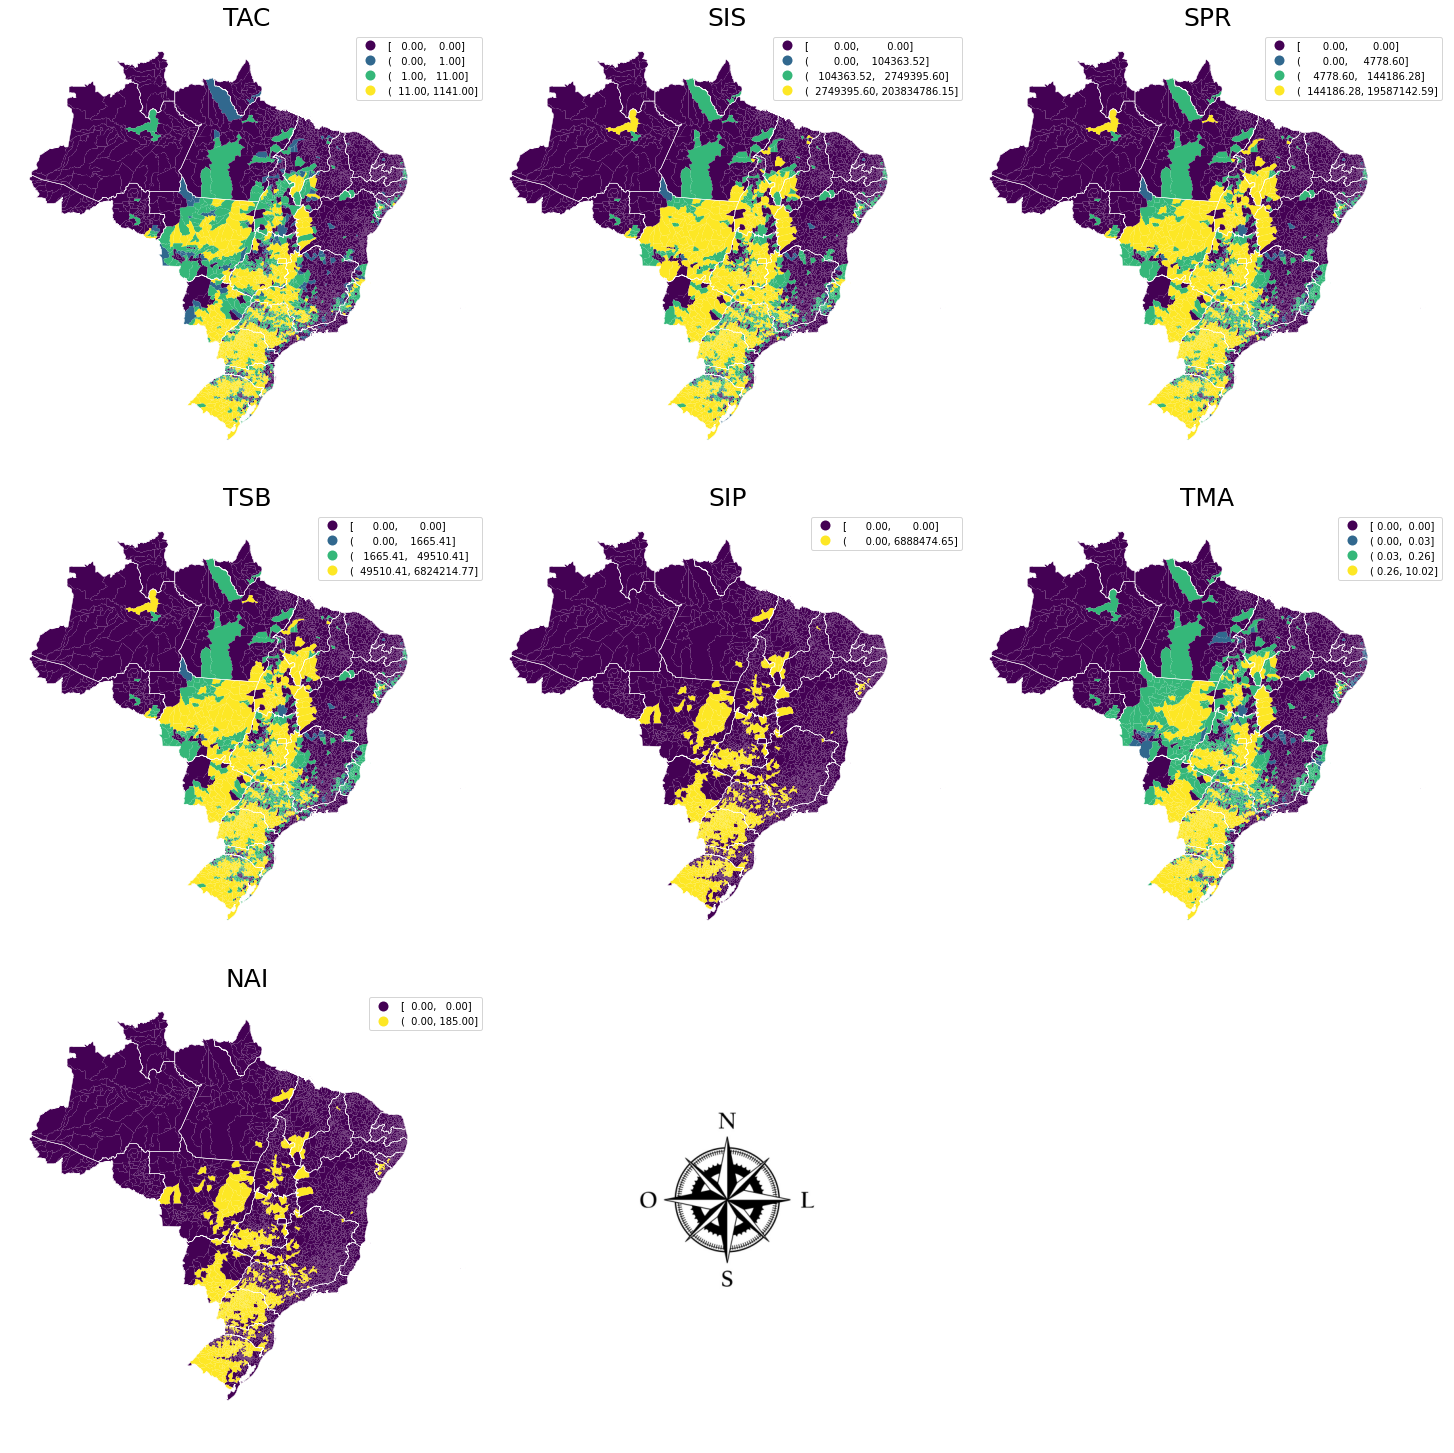
\includegraphics[width=0.4\textwidth]{img/map_variaveis.png}
    	\caption{Distribuição espacial das variáveis de seguro rural.}
    	\noindent \small \textsuperscript{Fonte: Elaboração própria}
    	\label{mapa_variaveis}
    \end{figure}
\end{frame}

\begin{frame}{Resultados -- Distribuição espacial}
    \begin{figure}[h]
    	\centering
    	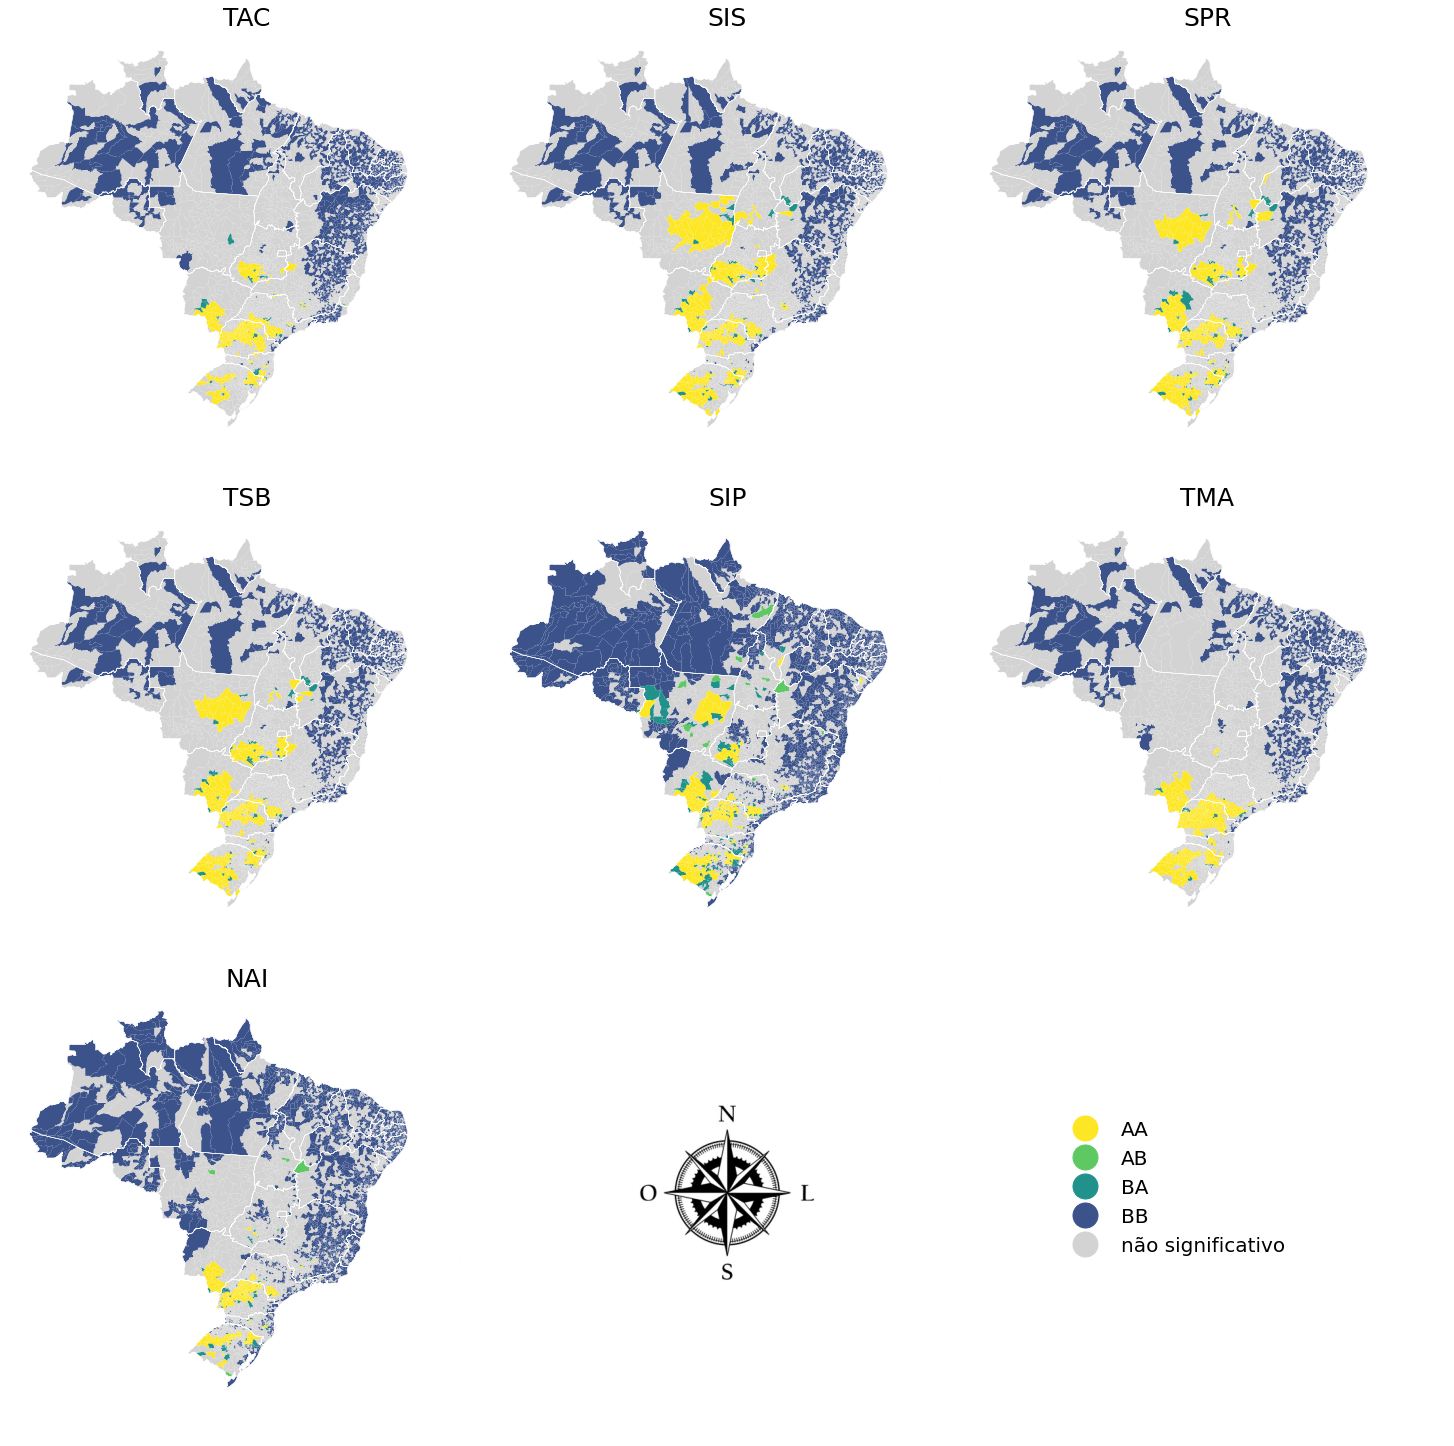
\includegraphics[width=0.4\textwidth]{img/map_i_moran_variaveis.png}
    	\caption{Distribuição espacial do \textit{I} de Moran local para as variáveis de seguro rural.}
    	\noindent \small \textsuperscript{Fonte: Elaboração própria}
    	\label{lisa_variaveis}
    \end{figure}
\end{frame}

\begin{frame}{Resultados -- Distribuição espacial}
    \begin{figure}[h]
    	\centering
    	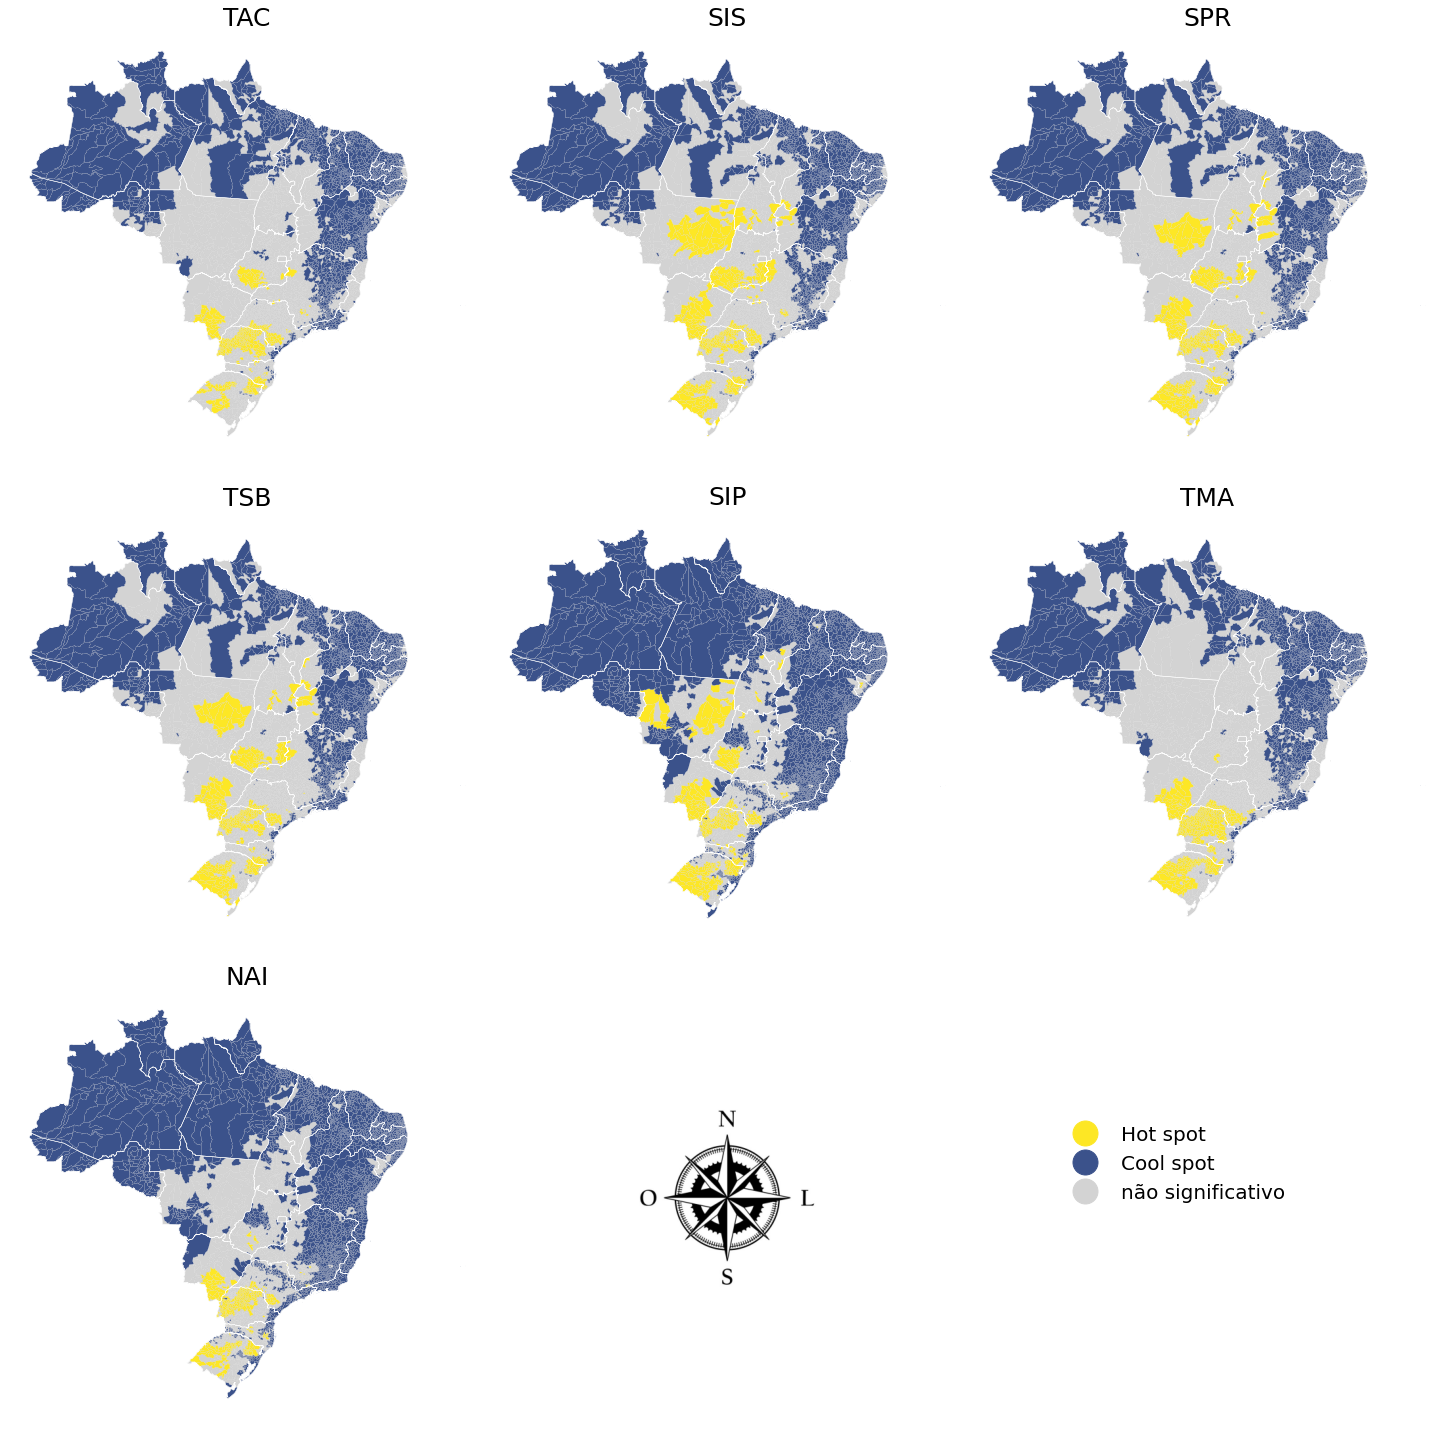
\includegraphics[width=0.4\textwidth]{img/map_getis_ord_variaveis.png}
    	\caption{Distribuição espacial do \textit{G} de Getis e Ord local para as variáveis de seguro rural.}
    	\noindent \small \textsuperscript{Fonte: Elaboração própria}
    \end{figure}
\end{frame}

\begin{frame}{Resultados -- Identificação dos agrupamentos}
	\begin{figure}
		\centering
		\footnotesize
		\subfloat[\textit{I} de Moran]{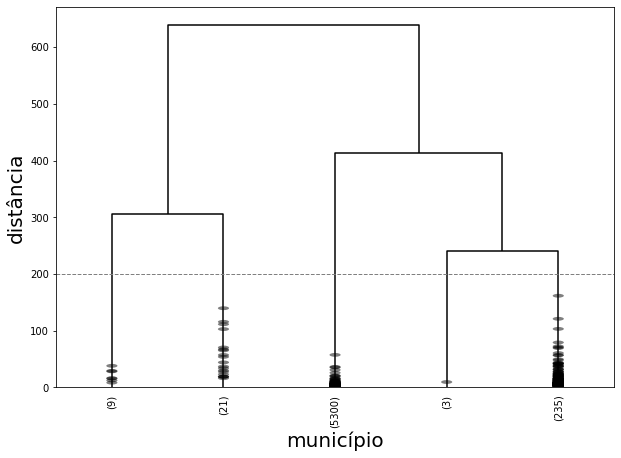
\includegraphics[width=0.4\textwidth]{img/dendrograma_i_moran.png}}
		\hspace{0.2cm}
		\subfloat[\textit{G} de Getis e Ord]{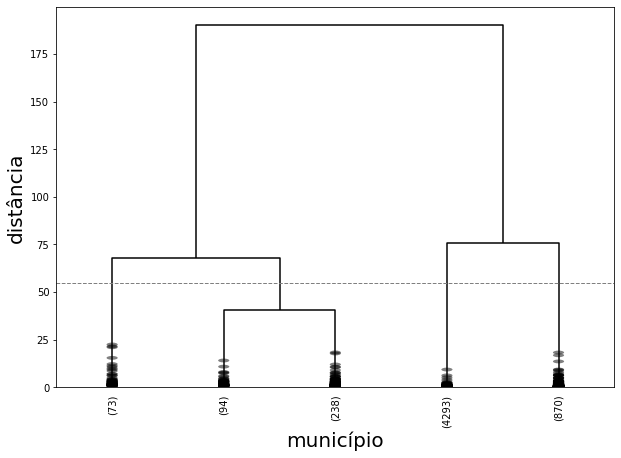
\includegraphics[width=0.4\textwidth]{img/dendrograma_getis_ord.png}}
    	\caption{Dendrogramas}\label{Dendrogramas}
	    \noindent \small \textsuperscript{Fonte: Elaboração própria}
	\end{figure}
\end{frame}


\begin{frame}{Resultados -- Identificação dos agrupamentos}
	\begin{figure}
		\centering
		\footnotesize
		\subfloat[\textit{I} de Moran]{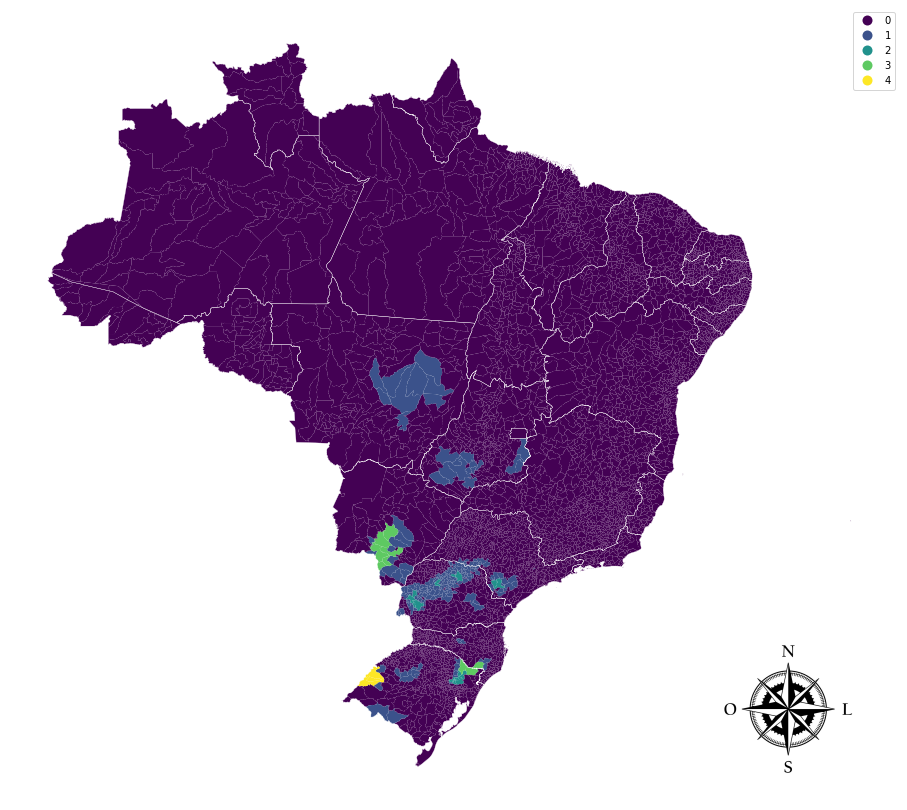
\includegraphics[width=0.4\textwidth]{img/grupos_ward_i_moran.png}}
		\hspace{0.2cm}
		\subfloat[\textit{G} de Getis e Ord]{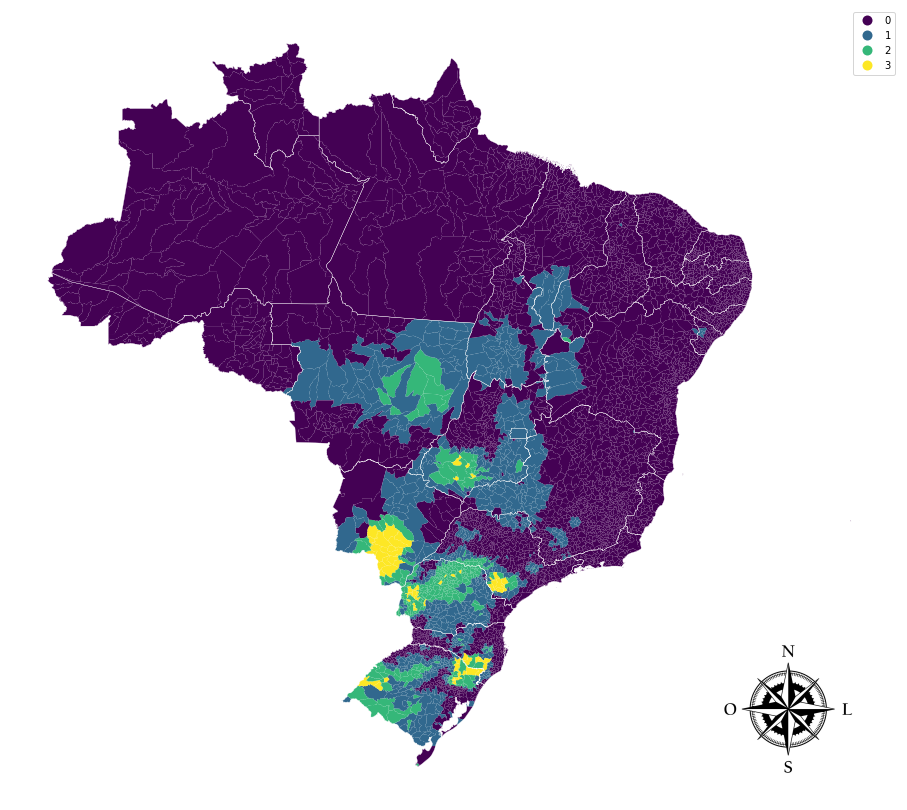
\includegraphics[width=0.4\textwidth]{img/grupos_ward_getis_ord.png}}
        \caption{Agrupamentos formados pelo método de \textit{Ward} com \textit{I} de Moran e \textit{G} de Getis e Ord}
        \noindent \small \textsuperscript{Fonte: Elaboração própria}
	\end{figure}
\end{frame}

\begin{frame}{Resultados -- Identificação dos agrupamentos}
	\begin{figure}
		\centering
		\footnotesize
		\subfloat[\textit{I} de Moran]{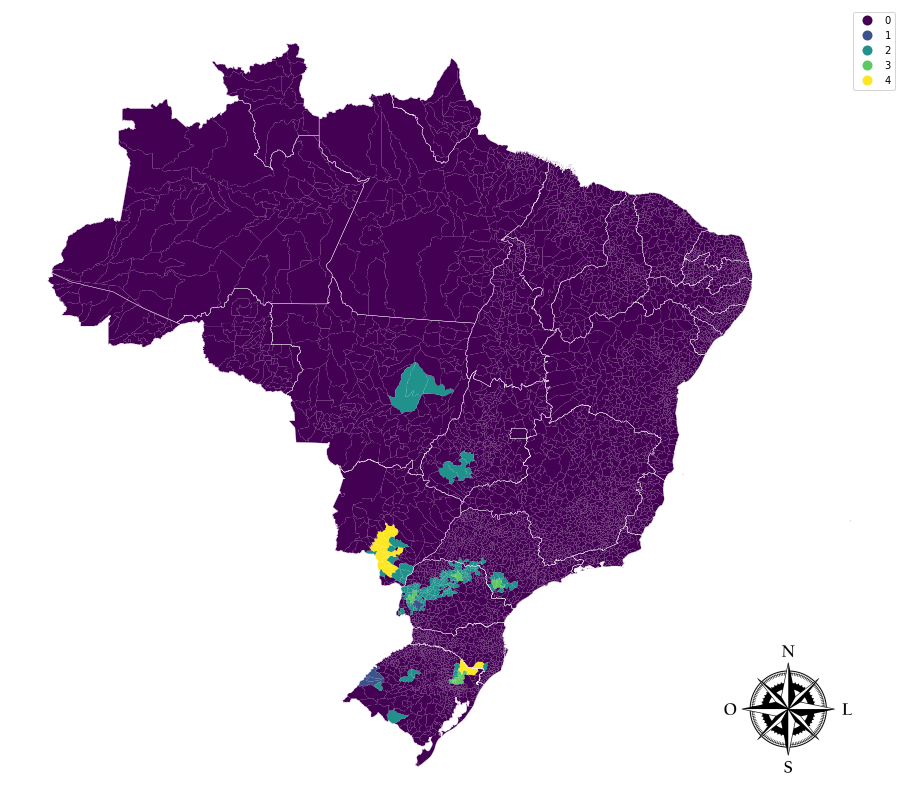
\includegraphics[width=0.4\textwidth]{img/grupos_kmedias_i_moran.png}}
		\hspace{0.2cm}
		\subfloat[\textit{G} de Getis e Ord]{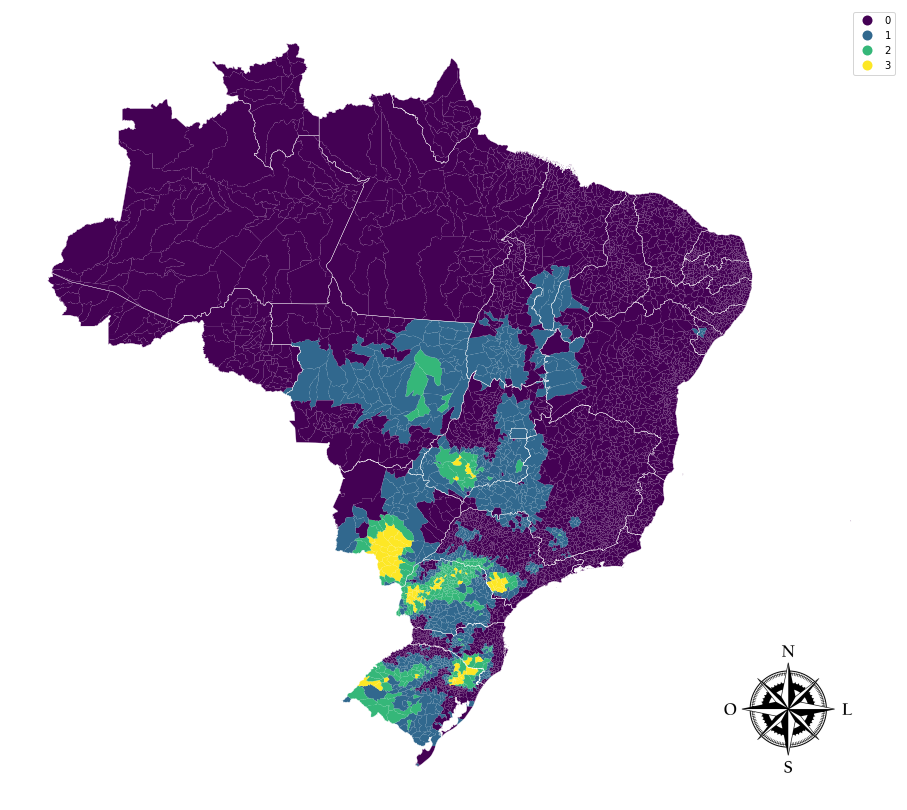
\includegraphics[width=0.4\textwidth]{img/grupos_kmedias_getis_ord.png}}
	    \caption{Agrupamentos formados pelo método das $k-$médias com \textit{I} de Moran e \textit{G} de Getis e Ord}\label{cluster_kmedia}
	    \noindent \small \textsuperscript{Fonte: Elaboração própria}
	\end{figure}
\end{frame}

\begin{frame}{Resultados -- Identificação dos agrupamentos}
    \begin{table}[h]
    \caption{Média da estatística $G_i$ nos grupos formados pelos métodos de \textit{Ward} e das  $k-$médias} \label{mean_G}
    \footnotesize
    \vspace{0.05cm}
    \begin{tabularx}{\textwidth}{LXXXXXXXX}
        \hline \\[-1.9ex]	 
        Método de agrupamento & Grupos & & & & Variáveis \\\cmidrule{3-9}
        
                              & & TAC   & SIS   & SPR   & TSB   & SIP  & TMA   & NAI   \\
        \hline \\[-1.9ex]	 
                         & 0 & -0,25 & -0,25 & -0,24 & -0,24 & -0,19 & -0,31 & -0,20 \\
        \textit{Ward}    & 1 &  0,34 &  0,56 &  0,42 &  0,42 &  0,31 &  0,54 &  0,18 \\
                         & 2 &  2,19 &  1,82 &  1,80 &  1,81 &  1,57 &  2,63 &  2,04 \\
                         & 3 &  4,29 &  4,56 &  4,90 &  4,91 &  3,70 &  3,37 &  3,13 \\
        \hline \\[-1,9ex]	 
                         & 0 & -0,23 & -0,23 & -0,22 & -0,22 & -0,18 & -0,29 & -0,19 \\
        $k-$médias       & 1 &  0,47 &  0,73 &  0,57 &  0,57 &  0,40 &  0,72 &  0,27 \\
                         & 2 &  4,43 &  4,22 &  4,40 &  4,41 &  3,61 &  3,65 &  3,60 \\
                         & 3 &  2,14 &  1,74 &  1,81 &  1,81 &  1,59 &  2,65 &  1,98 \\
        \hline 
    \end{tabularx} 
\end{table}
\noindent\footnotesize{Fonte: Elaboração própria.  }\\
\end{frame}

\begin{frame}{Resultados -- Identificação dos agrupamentos}
\begin{table}[h]
    \caption{Média da estatística \textit{I} de Moran nos grupos formados pelos métodos de \textit{Ward} e das  $k-$médias} \label{mean_I}
    \footnotesize
    \vspace{0.05cm}
    \begin{tabularx}{\textwidth}{LXXXXXXXX}
        \hline \\[-1.9ex]	 
        Método de agrupamento & Grupos & & & & Variáveis \\\cmidrule{3-9}
        
                      &   & TAC   & SIS   & SPR   & TSB   & SIP  & TMA   & NAI   \\
        \hline \\[-1.9ex]	 
                      & 0 &   0.11 &   0.12 &   0.09 &   0.09 &   0.08 &   0.26 &   0.11 \\
                      & 1 &   7.50 &   6.18 &   5.43 &   5.48 &   3.91 &  11.15 &   5.68 \\
        \textit{Ward} & 2 &  55.71 &  21.25 &  23.71 &  23.66 &  16.12 &  25.49 &  43.24 \\
                      & 3 &  14.16 &  44.68 &  62.54 &  64.17 &  11.47 &   7.50 &   4.27 \\
                      & 4 &   1.33 &  10.35 &  15.23 &  13.95 & 101.29 &   6.81 &   5.06 \\
        \hline \\[-1,9ex]	 
                      & 0 &   0,14 &   0,17 &   0,13 &   0,13 &   0,09  &   0,32 &   0,12 \\
                      & 1 &   6,23 &   8,65 &  12,17 &  11,43 &  82,02  &  14,88 &  25,84 \\
        $k-$médias    & 2 &  10,29 &   7,06 &   6,39 &   6,46 &   5,15  &  13,60 &   8,27 \\
                      & 3 &  65,42 &  25,53 &  29,04 &  28,90 &  13,88  &  28,56 &  45,68 \\
                      & 4 &  13,62 &  43,16 &  59,62 &  61,16 &  13,41  &   7,54 &   4,45 \\
        \hline 
    \end{tabularx} 
\end{table}
\noindent\footnotesize{Fonte: Elaboração própria.  }\\
\end{frame}

\subsection{Considerações finais}

\begin{frame}{Considerações finais}
	\begin{enumerate}
	    \item Os agrupamentos foram obtidos de forma a levar em consideração não apenas o valor das variáveis de seguro rural mas também seu posicionamento geográfico.
		\vspace{0.25cm}
		\item Ou seja, existem padrões de associação espacial estatisticamente significativos. Também foi possível identificar a presença de \textit{clusters} espaciais significativos.     	\vspace{0.25cm}
		\item  Identificou-se que as maiores concentrações de apólices de seguro rural estão situadas nas regiões Sul, Centro-Oeste e Sudeste, no sul do Estado de São Paulo
		\vspace{0.25cm}
		\item Municípios que possuem uma maior adesão ao seguro rural tendem a ser geograficamente próximos de municípios que também têm maior número de apólices de seguro rural contratadas
		\vspace{0.25cm}
	\end{enumerate}
\end{frame}

\section{Referências}

\begin{frame}{Referências}
	\begin{flushleft}
			\footnotesize{  

				{ALMEIDA, E. \textbf{Econometria Espacial Aplicada}. Campinas-SP: Alínea, 2012.}
				
				\vspace{0.2cm}
					
				{ANSELIN, L. Local indicatos of spatial association - LISA. \textbf{Geographical analysis}, v. 27, p. 93-115, 1995.}	

				\vspace{0.2cm}
				
				{CENTRO DE ESTUDOS AVANÇADOS EM ECONOMIA APLICADA (0CEPEA) \textbf{PIB do Agronegócio Brasileiro}. Disponível em: \url{https://www.cepea.esalq.usp.br/br/pib-do-agronegocio-brasileiro.aspx}. Acesso em: 26 jun 2021.}
				
				\vspace{0.2cm}
				
				{EVERITT, B.; HOTHORN, T. \textbf{An introduction to applied multivariate analysis with R.} Nova York: Springer-Verlag, 2011.}
				
				\vspace{0.2cm}
				
                {INSTITUTO BRASILEIRO DE GEOGRAFIA E ESTATÍSTICA - IBGE. \textbf{Censo Agropecuário 2017}. Rio de Janeiro, v. 8, p.1-105, 2019.}
                
                \vspace{0.2cm}
                
                {INSTITUTO BRASILEIRO DE GEOGRAFIA E ESTATÍSTICA - IBGE. \textbf{Malha Municipal}.  Disponível em: \url{https://ibge.gov.br/geociencias/organizacao-do-territorio/estrutura-territorial/15774-malhas.html?=&t=o-que-e} Acesso em: 18 out. 2020.}

				\vspace{0.2cm}
				
		    	{REY, S. J.; ANSELIN, L. PySAL: A Python library of spatial analytical methods.\textbf{ Review of Regional Studies}, v. 37, n. 1, p. 5–27, 2007.}
		    }
	\end{flushleft}
\end{frame}

\end{document}
